% \documentclass{article}
\documentclass[journal=jpclcd,manuscript=article]{achemso}
\usepackage[utf8]{inputenc}

% ALL: See "style guide" here: % https://docs.google.com/document/d/12xwId6RT73miifI1thtLL7c0GoVIXsSfZndO5bgdqag/edit#

% Tables
% Use Roman numerals for tables
% https://tex.stackexchange.com/a/226029
\usepackage[labelsep=period]{caption}
\captionsetup[table]{name=Table}
\renewcommand{\thefigure}{S\arabic{figure}}
\renewcommand{\thetable}{S\Roman{table}}
% \usepackage{multirow}

\usepackage{pdflscape}
\usepackage{textcomp}
\usepackage{gensymb}
\usepackage{geometry}
\usepackage{multirow}

\usepackage{subcaption} % For subfigures?

\usepackage{pifont}
\newcommand{\cmark}{\textcolor{blue}{\textrm{\ding{52}}}}%
\newcommand{\xmark}{\textcolor{red}{\textrm{\ding{56}}}}%

\usepackage{amsmath}
\usepackage{amssymb}
%usepackage{authblk}


% units
% \SI{X}{\UNIT} will write the value X with units \UNIT. 
% eg. \SI{30}{\celsius}
\usepackage{siunitx} 

\usepackage{graphicx}
\graphicspath{ {./images/} }

\setlength {\marginparwidth }{2cm}
\usepackage{todonotes}
\newcommand{\tino}[1]{\todo[inline,color=purple!40]{Tino: #1}}
\newcommand{\fbp}[1]{\todo[inline,color=orange!40]{Ferran: #1}}
\newcommand{\summary}[1]{\todo[inline,caption={},color=yellow!40]{Summary: \\ #1}}

\newcommand{\ssri}[1]{{
\fbox{
\parbox{0.8\textwidth}{  \fbox{$\triangleright$\textcolor{blue}{\textbf{Shashank}:}} 
#1
}}}}

\newcommand{\gbox}[1]{{
\fbox{
\parbox{0.8\textwidth}{  \fbox{$\triangleright$\textcolor{blue}{\textbf{Gon}:}} 
#1
}}}}

\newcommand{\pbox}[1]{{
\fbox{
\parbox{0.8\textwidth}{  \fbox{$\triangleright$\textcolor{blue}{\textbf{From Peter}:}} 
#1
}}}}

\newcommand{\pdebox}[1]{{
\fbox{
\parbox{0.8\textwidth}{  \fbox{$\triangleright$\textcolor{blue}{\textbf{From Philipp}:}} 
#1
}}}}

\newcommand{\editreadybox}[1]{{
\fbox{
\parbox{0.8\textwidth}{  \fbox{$\triangleright$\textcolor{green}{\textbf{READY TO EDIT}:}} 
#1
}}}}

\usepackage[normalem]{ulem}

\setlength{\textheight}{8.4in}
\setlength{\topmargin}{0.1in}
\setlength{\headheight}{0.2in}
\setlength{\headsep}{0.1in}
\setlength{\oddsidemargin}{0in}
\setlength{\textwidth}{6.5in}

\author{Peter M. Attia}
\email{peter.m.attia@gmail.com}
\affiliation{\scriptsize{Department of Materials Science and Engineering, Stanford University, Stanford, CA, USA}}
\author{Alexander Bills} 
\affiliation{Department of Mechanical Engineering, Carnegie Mellon University, Pittsburgh, PA, USA}
\author{Ferran Brosa Planella} 
\affiliation{WMG, University of Warwick, Coventry, UK, and Faraday Institution, Harwell, UK}
\author{Philipp Dechent} 
\affiliation{Institute for Power Electronics and Electrical Drives (ISEA), RWTH Aachen University, Aachen, Germany}
%%%%%%%%%%%%%%%%%%%%%%%%%%%%%%%%%%%%%%%%%%%%%%%%%%%%%%%%
\author{Gon\c{c}alo dos Reis} 
% Goncalo's ORCID: 0000-0002-4993-2672
\affiliation{School of Mathematics, University of Edinburgh, Edinburgh, UK and Centro de Matem\'atica e Aplica\c c$\tilde{\text{o}}$es (CMA), FCT, UNL, Caparica, Portugal}
%%%%%%%%%%%%%%%%%%%%%%%%%%%%%%%%%%%%%%%%%%%%%%%%%%%%%%%%
\author{Matthieu Dubarry}
\affiliation{Hawaii Natural Energy Institute, University of Hawaii at Manoa, Honolulu, HI, USA}
\author{Paul Gasper} 
\affiliation{National Renewable Energy Laboratory, Golden, CO, USA}
% %%%%%%%%%%%%%%%%%%%%%%%%%%%%%%%%%%%%%%%%%%%%%%%%%%%%%%%%
\author{Richard Gilchrist} 
% Richard's ORCID: 0000-0002-1606-2607
\affiliation{School of Mathematics, University of Edinburgh, Edinburgh, UK}
% %%%%%%%%%%%%%%%%%%%%%%%%%%%%%%%%%%%%%%%%%%%%%%%%%%%%%%%%
\author{Samuel Greenbank} 
\affiliation{Department of Engineering Science, University of Oxford, Oxford, UK}
\author{David Howey} 
\affiliation{Department of Engineering Science, University of Oxford,  Oxford, UK, and Faraday Institution, Harwell, UK}
\author{Ouyang Liu} 
\affiliation{Institute for Infocomm Research, Agency for Science, Technology, and Research (A*STAR), Connexis, Singapore}
\author{Edwin Khoo}  
\affiliation{Institute for Infocomm Research, Agency for Science, Technology, and Research (A*STAR), Connexis, Singapore}
\author{Yuliya Preger}  
\affiliation{Sandia National Laboratories, Albuquerque, NM, USA}
\author{Abhishek Soni}
\affiliation{Department of Mechanical Engineering, University of Cincinnati, Cincinnati, OH, USA}
\author{Shashank Sripad} 
\affiliation{Department of Mechanical Engineering, Carnegie Mellon University, Pittsburgh, PA, USA}
\author{Anna G. Stefanopoulou}  
\affiliation{Department of Mechanical Engineering, University of Michigan, Ann Arbor, MI, USA}
\author{Valentin Sulzer}
\affiliation{Department of Mechanical Engineering, University of Michigan, Ann Arbor, MI, USA}


\title{
{\large{\bfseries{Supplementary Information for}}} \\ \Large\bfseries
``Knees'' in lithium-ion battery aging trajectories}

 \date{}
%  \date{\today}
 
 
 
\begin{document}
\maketitle
\thispagestyle{empty}


 %
 
 
 
 %%%%%%%%%%%%%%%%%%%%%%%%%%%%%%%%%%%%%%%%%%%%%%%%%
 %%%%%%%%%%%%%%%%%%%%%%%%%%%%%%%%%%%%%%%%%%%%%%%%%

\section{Supplementary Discussion 1. Knees across identification algorithms}

Figure \ref{fig:severson_knee_eol_all_algorithms} presents linear regressions of knee-point to end-of-life for the capacity curves of the Severson et al. \cite{severson_data-driven_2019} dataset across the knee identification algorithms discussed (except the Zhang et al.\cite{zhang_identifying_2020} method). We mention that there is no ``ground truth'' for the true knee. For the Bacon-Watts and Kneedle identified knees, the linear regression holds with a goodness-of-fit $R^2\approx 99\%$ (and reduced variance between fit and residuals). With this metric, close by is the bisector\cite{greenbank_automated_nodate} identified knees with $R^2\approx 96\%$. The tangent-ratio\cite{diao_algorithm_2019} identified knees show a higher fit-to-residuals variability.  

\begin{figure}[ht]
\centering
% \begin{subfigure}{.5\textwidth}
%   \centering
% 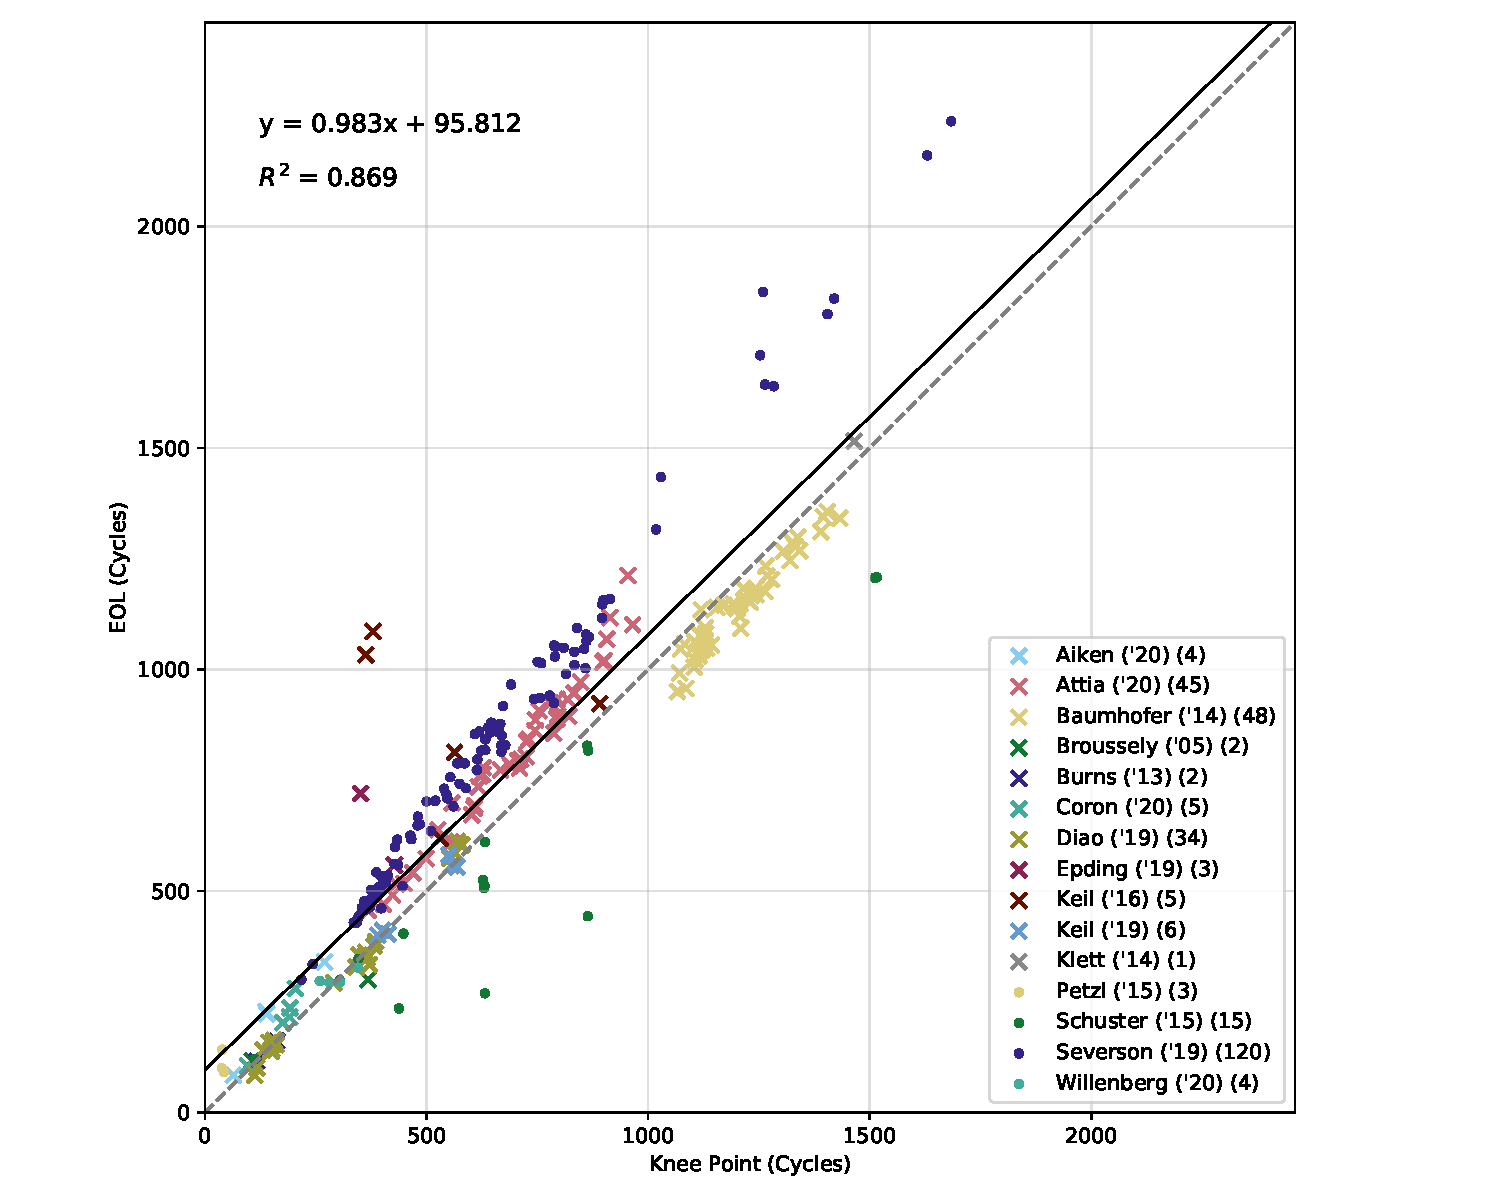
\includegraphics[scale=0.70]{figures/AcrossDatasetsknee-to-EOL}
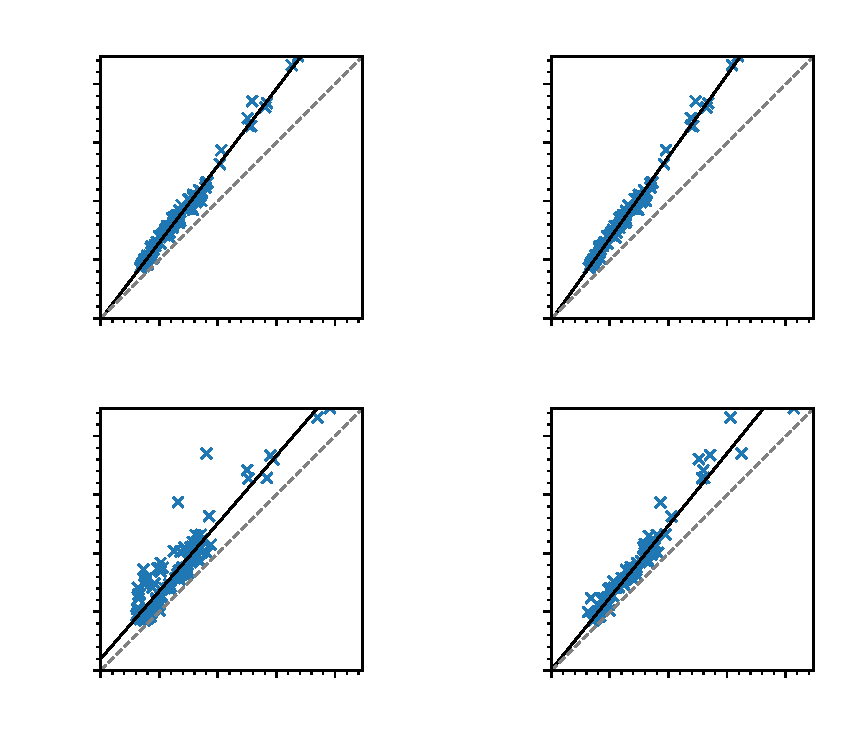
\includegraphics[scale=1.0]{figures/severson_knee_eol_all_algorithms.eps}
%   \caption{Linear regression of knee-point to EOL point}
  \label{fig:kneepoint2EOL}
% \end{subfigure}%
\caption{Linear relationship between identified knees and end-of-life (EOL) per knee identification algorithm over the Severson et al. \cite{severson_data-driven_2019} dataset. (a) Bacon-Watts\cite{fermin-cueto_identification_2020}, (b) Kneedle\cite{satopaa_finding_2011}, (c) Tangent-ratio\cite{diao_algorithm_2019}, (d) Bisector\cite{greenbank_automated_nodate}.
}.
\label{fig:severson_knee_eol_all_algorithms}
\end{figure}

%%%%%%%%%%%%%%%%%%%%%%%%%%%%%%%%%%%%%%%%%
%%%%%%%%%%%%%%%%%%%%%%%%%%%%%%%%%%%%%%%%%%%%%%%%%

\section{Supplementary Discussion 2. Impact of $x$ axis visualization choice on knee onset}

Capacity fade plots are typically presented with a cycle-based axis; however, this choice may obscure the influence of calendar aging phenomena. The influence of time is most notable for the study of variables like charge/discharge rate and rest time. 
In Figure \ref{fig:discharge-rest_time}, we replotted the data in Figure \textbf{18} 
%\ref{fig:discharge-rest_cycle} 
with a time-based axis instead of a cycle number-based axis. Raw data from the corresponding studies were not available, so the cycle times were estimated from the given C rates and rest times. The trends in discharge rate and rest time influence on knee onset are largely the same as in the cycle-based figure. However, the change from Figure 18c
%  \ref{fig:discharge-rest_cycle}c
to Figure \ref{fig:discharge-rest_time}c suggests that much of the reason that longer rest times at top-of-charge and bottom-of-discharge decrease cycle life (at least in this study) is calendar aging, not greater degradation at the voltage extremes.    

\begin{figure}[ht]
\centering
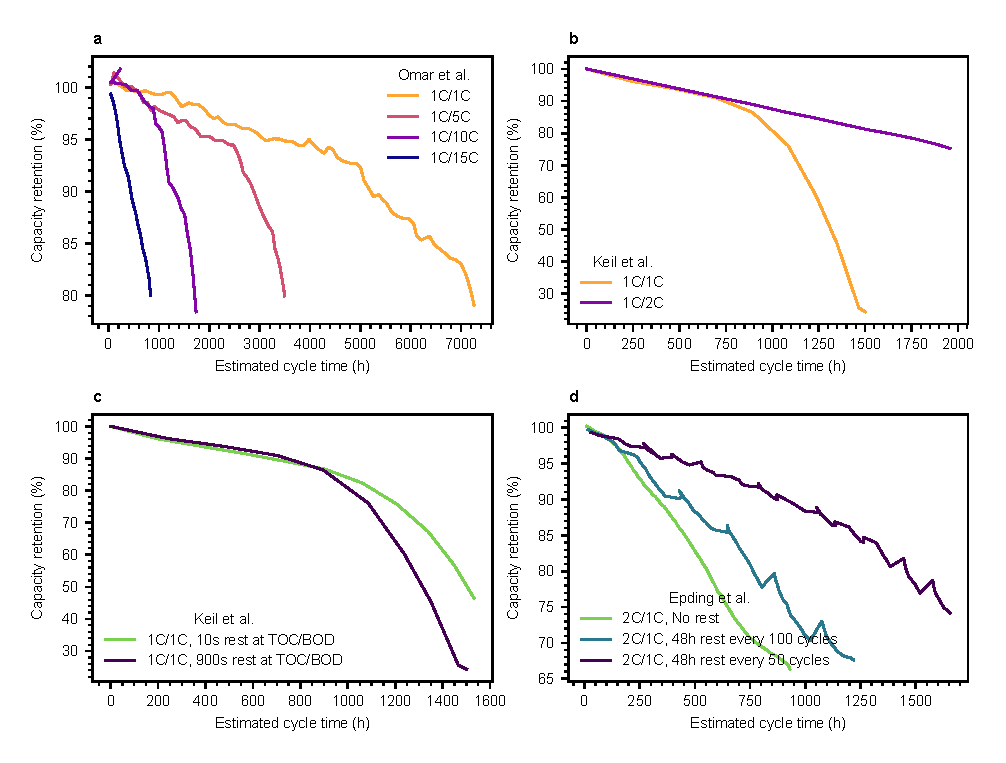
\includegraphics[scale = 1.0]{figures/discharge_rate_rest_time.eps}
\caption{Mixed effects of discharge rate and rest time on knee onset, depending on the testing conditions.
Data replotted from Figure \textbf{X} with a time-based $x$ axis (estimated from C rates).
(a) Higher discharge rate can accelerate knee onset. Adapted from Figure 8 of Omar et al.\cite{omar_lithium_2014} (b) Lower discharge rate can accelerate knee onset. Adapted from Figure 2a of Keil et al.\cite{keil_linear_2019} (c) Longer rest time can accelerate knee onset. Adapted from  Figure 2a of Keil et al.\cite{keil_linear_2019} (d) Shorter rest time can accelerate knee onset. Adapted from Figure 1a of Epding et al.\cite{epding_investigation_2019}.}
\label{fig:discharge-rest_time}
\end{figure}







%%%%%%%%%%%%%%%%%%%%%%%%%%%%%%%%%%%%%%%%%
%%%%%%%%%%%%%%%%%%%%%%%%%%%%%%%%%%%%%%%%%%%%%%%%%

% \gbox{refer to Yulia's table "SI-EXP Table"// Table \ref{table:experimental_summary}},

\newgeometry{margin=2.5cm}
\begin{landscape}
\begin{table}[p]
\caption{Summary of references used to generate Figure \textbf{20} in the main manuscript.
The data was obtained extracted via direct access to the corresponding databases when possible \cite{baumhofer_production_2014,diao_accelerated_2019,severson_data-driven_2019,willenberg_high-precision_2020,attia_closed-loop_2020} or via \textit{WebPlotDigitizer}\cite{dos_reis_lithium-ion_2021}.}
\label{table:experimental_summary_DATASOURCES}
\scalebox{0.5}{
\begin{tabular}{|c|c|l|l|l|c|l|}
\hline
\multicolumn{1}{|l|}{} & \multicolumn{1}{l|}{\textbf{Variable}} & \textbf{Reference} & \textbf{Cell Description} & \textbf{Range of Variable} & \textbf{Number of cells} & \textbf{Capacity curve references} \\ \hline
\multirow{9}{*}{\textbf{Cell design}} & \textbf{Electrode loading} & Ma et al. 2019 \cite{ma_editors_2019} & Lab-made pouch NMC/Gr & 14.4--21.2 mg/cm2 & &  
\\ \cline{2-7} 
 & 
%  \textbf{Positive electrode coating} 
 \begin{tabular}[c]{@{}l@{}} \textbf{Positive electrode}\\ \textbf{coating}\end{tabular}
 & Ma et al. 2019 \cite{ma_editors_2019} & Lab-made pouch NMC/Gr & Ti-based coating &  &  
 \\ \cline{2-7} 
 & \textbf{Graphite type} & Ma et al. 2019 \cite{ma_editors_2019} & Lab-made pouch NMC/Gr & Artificial (Kaijin AML-400), natural (BTR-918) &  & 
 \\ 
 \cline{2-7} 
 & \multirow{3}{*}{
%  \textbf{Additive package and concentration}
 \begin{tabular}[c]{@{}l@{}} \textbf{Additive package}\\ \textbf{and concentration}\end{tabular}
  } & Petibon et al. 2016 \cite{petibon_studies_2016} & Lab-made pouch LCO/Gr-Si & N/A &   &   
  \\ 
 \cline{3-7} 
 &  & Jung et al. 2016 \cite{jung_consumption_2016} & Lab-made coin LFP/Gr-Si & 0--20 wt.\% FEC &   &   
 \\ 
 \cline{3-7} 
 &  & Ma et al. 2019 \cite{ma_editors_2019} & Lab-made pouch NMC/Gr & 0--20\% methyl acetate additive &   &   \\ 
 \cline{2-7} 
 & \multirow{3}{*}{\textbf{Salt concentration}} & Aiken et al. 2020 \cite{aiken_accelerated_2020} & Lab-made pouch NMC/Gr & 0.2--1.2M LiPF6 & 4 & 
 \begin{tabular}[c]{@{}l@{}} Fig 3d 0.8M, 1.2M;\\ Fig 10a: 'red circle' and 'blue circle' \end{tabular}
  \\ 
 \cline{3-7} 
 &  & Ma et al. 2019 \cite{ma_editors_2019} & Lab-made pouch NMC/Gr & 1.2--1.5M LiPF6 &   & 
 \\ 
 \cline{3-7} 
 &  & Wang et al. {[}x{]} & Lab-made pouch LCO/Gr & 0.5--2M LiPF6 &  &  
 \\ 
 \hline
\multirow{34}{*}{%\textbf{Testing Conditions}
\begin{tabular}[c]{@{}l@{}} \textbf{Testing}\\ \textbf{conditions}\end{tabular}
} & \multirow{8}{*}{\textbf{Charging rate}} & Lewerenz et al. 2017 \cite{lewerenz_systematic_2017}, \cite{lewerenz_post-mortem_2017} & OMT OMLIFE-8AH-HP LFP/Gr & 1--8C &  & 
\\ \cline{3-7} 
 &  & Petzl et al. 2015 \cite{petzl_lithium_2015} & Commercial 26650 LFP/Gr & 0.5--1C &  & 
 \\ 
 \cline{3-7} 
 &  & Burns et al. 2015 \cite{burns_-situ_2015} & Panasonic 18650 NCA/Gr & 0.1--1C & 2 & Fig1b circles and squares \\ 
 \cline{3-7} 
 &  & Waldmann et al. 2015 \cite{waldmann_optimization_2015} & Cylindrical NCA/Gr & 0.25--1C, single vs. multi-step CC, optional CV &   & 
 \\ 
 \cline{3-7} 
 &  & Schuster et al. 2015 \cite{schuster_nonlinear_2015} & E-One Moli Energy IHR18650A NMC/Gr & 0.2--1C & 15 & 
  \begin{tabular}[c]{@{}l@{}}  
  Fig 1a; Fig 4a 1.30V (CCCV) (A); Fig 4a 1.20V (CCCV) (A);  \\
 Fig 4a 1.20V (CC) (A); Fig 4a 0.94V (CC) (A);   \\
 Fig 6a 0.5C/0.5C (A); Fig 6a 1.0C/0.5C (A); Fig 6a 0.5C/1.0C (A);   \\
 Fig 9 1.20 V (CC); Fig 9 1.20 V (CCCV); Fig 9 1.20 V (2CCCV); \\
 Fig 10a 35degC(deltaV down) (A); Fig 10a 35degC(deltaV up) (A); \\
 Fig 10a 50degC(deltaV up) (A); Fig 10a 25degC(deltaV up) (A);  \end{tabular}
 \\ 
 \cline{3-7} 
 &  & Severson et al. 2019 \cite{severson_data-driven_2019} & A123 APR18650M1A LFP/Gr & 3.6--8C & 120 & Database access 
 \\ 
 \cline{3-7} 
 &  & Schindler et al. 2018 \cite{schindler_fast_2018} &  Samsung ICR18560-26F NMC/Gr & 
%  0.25-2C with AC pulse, current derating, current interrupt
  \begin{tabular}[c]{@{}l@{}}0.25--2C with AC pulse, \\ current derating, current interrupt\end{tabular}
 & &   
 \\ 
 \cline{3-7} 
 &  & 
 Keil et al. 2019 \cite{keil_linear_2019} & Cylindrical NMC/Gr & 0.7--1C & 6 & 
   \begin{tabular}[c]{@{}l@{}}  
Fig 2a procedure 1 and 2; Fig 8a procedure 1 100 SOC;  \\
Fig 8a procedure 1 0 SOC; Fig 8a procedure 2 100 SOC;   \\
Fig 8a procedure 2 0 SOC  \end{tabular}
 \\ 
 \cline{2-7} 
 & \multirow{5}{*}{\textbf{Discharging rate}} & 
 Keil et al. 2016 \cite{keil_charging_2016} & \begin{tabular}[c]{@{}l@{}}a) Sanyo UR18650SA LMO+NMC/Gr\\ b) Sony US18650VT1 LMO+LCO/Gr\\ c) A123 APR18650M1A LFP/Gr\end{tabular} 
 & \begin{tabular}[c]{@{}l@{}}a) 2.4--4C\\ b) 2.7--4.5C\\ c) 2.7--4.5C\end{tabular} & 5 & 
  \begin{tabular}[c]{@{}l@{}}Fig 8c 3A CCCV +50mV (C); Fig 10a 1A CCCV (A);\\ Fig 10a 1A CCCV (A); Fig 10b 3A CCCV (B);\\ Fig 10c 5A CCCV (C) \end{tabular}
  \\ 
 \cline{3-7} 
 &  & 
 Keil et al. 2019 \cite{keil_linear_2019} & Cylindrical NMC/Gr & 1--2C & see above & see above \\ 
 \cline{3-7} 
 &  & Atalay et al. 2020 \cite{atalay_theory_2020} & Commercial 18650 NCA/Gr & 1--4C &   &   
 \\ 
 \cline{3-7} 
 &  & Omar et al. 2014 \cite{omar_lithium_2014} & Commercial cylindrical LFP/Gr & 1--15C &   &   
 \\ 
 \cline{3-7} 
 &  & Diao et al. 2019 \cite{diao_accelerated_2019} & Pouch LCO/Gr & 0.7--2C & 34 &  Database access
 \\
 \cline{2-7} 
 & \multirow{8}{*}{\textbf{Voltage limits}} & Broussely et al. 2005 \cite{broussely_main_2005} & Saft VLE NCA/Gr & 50\%--100\% storage SOC & 2 &  Fig 2 red and green 
 \\ 
 \cline{3-7} 
 &  & Aiken et al. 2020 \cite{aiken_accelerated_2020} & Lab-made pouch NMC/Gr & 4.3--4.4V charge cutoff voltage &  & 
 \\ 
 \cline{3-7} 
 &  & 
 \begin{tabular}[c]{@{}l@{}} Ecker et al. 2014 \cite{ecker_calendar_2014},\\ Pfrang et al. 2018 \cite{pfrang_long-term_2018}\end{tabular}
%  Ecker et al. 2014 \cite{ecker_calendar_2014}, Pfrang et al. 2018 \cite{pfrang_long-term_2018} 
 & Sanyo UR18650E NMC/Gr & \begin{tabular}[c]{@{}l@{}}1) 0.5\%--100\% DOD, 50\% SOC midpoint\\ 2) 10\% DOD and midpoint SOC of 10\%--95\%\end{tabular} &  &  
 \\ 
 \cline{3-7} 
 &  & Klett et al. 2014 \cite{klett_non-uniform_2014} & Commercial 26650 LFP/Gr & 30--50\% vs. 5--95\% SOC & 1 & Figure 2a CCC \\ 
 \cline{3-7} 
 &  & Schuster et al. 2015 \cite{schuster_nonlinear_2015} & E-One Moli Energy IHR18650A NMC/Gr & 0.56--1.2V DOD, 3.6V midpoint & See above & See above \\ 
 \cline{3-7} 
 &  & Ma et al. 2019 \cite{ma_novel_2019} & Commercial prismatic NMC+LMO/Gr & 0--20\%, 20--60\%, 60--100\%, 0--100\% SOC &  & \\ 
 \cline{3-7} 
 &  & Petzl et al. 2015 \cite{petzl_lithium_2015} & Commercial 26650 LFP/Gr & 0--80\% vs. 0--100\% SOC & 3 & Fig 1a blue, red, black 
 \\ 
 \cline{3-7} 
 &  & Zhu et al. 2021 \cite{zhu_investigation_2021} & Samsung INR 18650 25R NMC+NCA/Gr & 20--60\% DOD, 15--85\% SOC midpoint &  &  
 \\ 
 \cline{2-7} 
 & \multirow{3}{*}{\textbf{Rests}} & Keil et al. 2019 \cite{keil_linear_2019} & Cylindrical NMC/Gr & 10--900s at TOC and BOD & See above & See above \\ 
 \cline{3-7} 
 &  & Ma et al. 2019 \cite{ma_editors_2019} & Lab-made pouch NMC/Gr & 0--30min at TOC and BOD &   & 
 \\ 
 \cline{3-7} 
 &  & Epding et al. 2019 \cite{epding_investigation_2019} & Commercial prismatic NMC/Gr & 0--every 100 cycles & 3 & Fig 1a black and green; Fig 7a black cell 2
 \\ 
 \cline{2-7} 
 & \multirow{7}{*}{\textbf{Temperature}} & Zhang et al. 2019 \cite{zhang_accelerated_2019} & NMC/Gr & 25--45\degree C &  &  
 \\ 
 \cline{3-7} 
 &  & Broussely et al. 2005 \cite{broussely_main_2005} & Saft VLE NCA/Gr & 20--60C & &  
 \\ \cline{3-7} 
 &  & Schuster et al. 2015 \cite{schuster_nonlinear_2015} & E-One Moli Energy IHR18650A NMC/Gr & 25--50\degree C & See above & See above \\ 
 \cline{3-7} 
 &  & Safari et al. 2011 \cite{safari_aging_2011} & Commercial 26650 LFP/Gr & 25--45\degree C &   &   
 \\ 
 \cline{3-7} 
 &  & Waldmann et al. 2014 \cite{waldmann_temperature_2014} & Commercial 18650 NMC+LMO/Gr & -20--70\degree C &   &   \\ 
 \cline{3-7} 
 &  & Coron et al. 2020 \cite{coron_impact_2020} & \begin{tabular}[c]{@{}l@{}}Commercial 18650 NMC+LMO/Gr\\  Commercial 18650 NMC/Gr\end{tabular} & 0--25\degree C & 5 &  
 \begin{tabular}[c]{@{}l@{}}Fig 1c: 'red crosses', 'red squares',\\ 'blue crosses', 'blue squares' and  'blue circles' \end{tabular}
 \\ 
 \cline{3-7} 
 &  & Waldmann et al. 2015 \cite{waldmann_optimization_2015} & Cylindrical NCA/Gr & 0--60\degree C & & 
 \\ 
 \cline{2-7} 
 & \multirow{3}{*}{\textbf{Pressure}} & Wunsch et al. 2019 \cite{wunsch_investigation_2019} & Commercial pouch NMC/Gr & 4 bracing approaches &  &  \\ 
 \cline{3-7} 
 &  & Cannarella et al. 2014 \cite{cannarella_stress_2014} & Pouch LCO/Gr & 0--5 MPa & & 
 \\ \cline{3-7} 
 &  & Bach et al. 2016 \cite{bach_nonlinear_2016} & E-One Moli Energy IHR18650A NMC/Gr & With and without hose clamp &  & \\ 
 \hline
\multirow{4}{*}{%\textbf{Cell-to-cell Variation}
\begin{tabular}[c]{@{}l@{}} \textbf{Cell-to-cell}\\ \textbf{variation}\end{tabular}
} & \multicolumn{1}{l|}{\multirow{4}{*}{\textbf{}}} & Harris et al. 2017 \cite{harris_failure_2017} & Commercial pouch LCO/Gr & 24 cells &  &  \\ 
\cline{3-7} 
 & \multicolumn{1}{l|}{} & Baumhofer et al. 2014 \cite{baumhofer_production_2014} & Sanyo UR18650E NMC/Gr & 48 cells & 48 & Database access \\ 
 \cline{3-7} 
 & \multicolumn{1}{l|}{} & Willenberg et al. 2020 \cite{willenberg_high-precision_2020} & Samsung INR18650 35E NCA/Gr+Si & 4 cells & 4 & Database access \\ 
 \cline{3-7} 
 & \multicolumn{1}{l|}{} & Stiaszny et al. 2014 \cite{stiaszny_electrochemical_2014} & Commercial 18650 NMC+LMO/Gr & 6 cells &  &  \\ 
 \hline
\end{tabular}
}
\end{table}

\end{landscape}
 \restoregeometry










%%%%%%%%%%%%%%%%%%%%%%%%%%%%%%%%%%%%%%%%%%%%%%
%%%%%%%%%%%%%%%%%%%%%%%%%%%%%%%%%%%%%%%%%%%%%%%%%%%%
%%%%%%%%%%%%%%%%%%%%%%%%%%%%%%%%%%%%%%%%%%%%%%%%%%%%%%%%%
% \bibliographystyle{myIEEEtran}
\bibliography{refs_zotero}

\end{document}